\chapter{Fundamentação Teórica}
Este capítulo apresenta uma visão geral sobre linha de produto de \textit{software},
gerência de variabilidades na plataforma Android, padrões de projeto e orientação
a objetos e um \textit{framework} para comparação de técnicas de implementação
de variabilidades.

\section{Linha de Produto de Software}

Linha de produto de \textit{software} é uma família de \textit{softwares} que possuem um núcleo
comum e que possibilita personalizações para cada produto específico \cite{Clements2001}.
Cada produto é criado a partir das variabilidades permitidas para a linha de produto.
Podendo ser de dois tipos: (i) variabilidades de negócio e (ii) variabilidades de
plataforma.
As primeiras são adaptações em requisitos de negócios da aplicação requeridas pelo
usuário final.
As últimas dizem respeito às variações no ambiente de hardware e software em que
uma aplicação será executada. Está intrinsecamente ligada a aspectos técnicos
relacionados ao dispositivo no qual a aplicação está instalada. Assim, uma
importante disciplina na engenharia de linha de produto de \textit{software} é a
gerencia de variabilidades.

\subsection{Gerência de Variabilidades}

Gerência de variabilidades está relacionado às atividades de suporte a variabilidades
no ciclo de vida do software, permitindo o gerenciamento de dependências e interações
entre variabilidades. Técnicas de gerência de variabilidades permitem sistematicamente
desenvolver e evoluir artefatos comuns e variáveis pertencentes a uma LPS.

\subsubsection{Variabilidades de Negócios}
Variabilidades de negócio são adaptações em requisitos de negócio da aplicação
requerida pelo usuário final. Em geral, gerentes de produto de aplicações são
responsáveis por decidir quais variabilidades de negócio uma LPS pretende oferecer
suporte. O usuário final é responsável por escolher quais variabilidades estarão
presentes nos produtos desejados. Existem diferentes soluções para implementar
variabilidades de negócio. Variabilidades alternativas que podem funcionar com
determinados produtos, por exemplo, podem ser implementadas através do uso dos
mecanismos de herança e polimorfismo de orientação a objetos, permitindo que
classes abstratas sejam estendidas para oferecer implementações específicas para
um dado produto. Padrões de projeto orientados a objetos \cite{Gamma1994} podem ser
aplicados dentro deste contexto, oferecendo implementações modularizadas para
cada uma das variantes de uma variabilidade específica. Em tais soluções, a escolha
de quais variantes serão selecionadas é delegada para uma ferramenta de derivação
de produto, a qual se responsabiliza pela inclusão das subclasses específicas
responsáveis pela inclusão no produto final.

\subsubsection{Variabilidades de Plataforma}
Plataforma refere-se ao ambiente de hardware e software em que uma aplicação irá
ser executada \cite{Preuveneers2004}. Assim, variabilidades de plataforma dizem
respeito a variações
de elementos desse conjunto. Ela está intrinsecamente ligada a aspectos técnicos
relacionados ao dispositivo no qual a aplicação é instalada, tais como:
implementações alternativas para versões que utilizam diferentes bibliotecas de classes
(APIs) e ajuste de \textit{layout} de telas para diferentes dispositivos.

\section{Gerência de Variabilidades na Plataforma Android}

Esta seção introduz técnicas de gerência de variabilidades disponíveis na plataforma
Android. Uma variabilidade refere-se à habilidade das aplicações adaptarem seu comportamento
para uso em um contexto particular. Considerando a produção em massa de aplicações móveis
para Android, pode se identificar duas forças predominantes que orientam a necessidade
por adaptações. A primeira é a imensa variedade de dispositivos existentes. Aplicações
móveis para Android devem ser capaz de fornecer a mesma experiência de usuário em
diferentes tipos de dispositivos. Por exemplo, toda aplicação móvel deve adaptar
sua interface de usuário de acordo com as configurações de tela disponíveis. Além
disso, elas devem também garantir que o layout correto são aplicados para as telas
corretas. A segunda são as necessidades específicas dos usuários. Atualmente, o
crescente número e diversidade de usuários demanda por aplicações personalizadas.

As seções seguintes apresentam como variabilidades de plataforma podem ser atendidas
em aplicações presentes na plataforma Android.

\subsection{Variabilidades de Plataforma}

\subsubsection{Versão da API}

Cada versão da plataforma geralmente adiciona novas funcionalidades, não previstas
em versões anteriores, ou muda a maneira de interação com o usuário. Nesse caso,
a plataforma permite que sejam declarados a versão mínima da API com qual sua
aplicação é compatível. Também é possível descobrir em tempo de execução qual a
versão da API está disponível no dispositivo e, assim, fazer algum tratamento diferenciado.

Android provê uma plataforma de aplicação dinâmica que oferece suporte para recursos
específicos por configuração, como declarar que um dispositivo de hardware é necessário
ou qual a versão mínima da API. Quando um usuário encontra um aplicativo de seu interesse
na Google Play Store, automaticamente é determinado se o aplicativo é ou não compatível
com o dispositivo. Quando o dispositivo não provê as funcionalidades necessárias,
o usuário não poderá instalar a aplicação. Embora seja possível a instalação manual
caso o usuário possua o arquivo de instalação da aplicação. Também é possível descobrir
em tempo de execução se algum recurso está ou não presente no dispositivo e, assim,
fazer algum tratamento diferenciado.

A figura \ref{fig:platform_versions} informações da distribuição por versão da plataforma.
Cada versão do Android recebe uma numeração de versão (coluna Version na tabela
presente na figura), um apelido (coluna Codename) e um número inteiro que representa
versão da API (coluna API). Esses valores representando os dispositivos com Android
que acessaram a Google Play Store nos 7 dias anteriores a 1º de agosto de 2016 e
versões com uso interior a 0,1\% não são exibidos. 

\begin{figure}[ht]
\centering
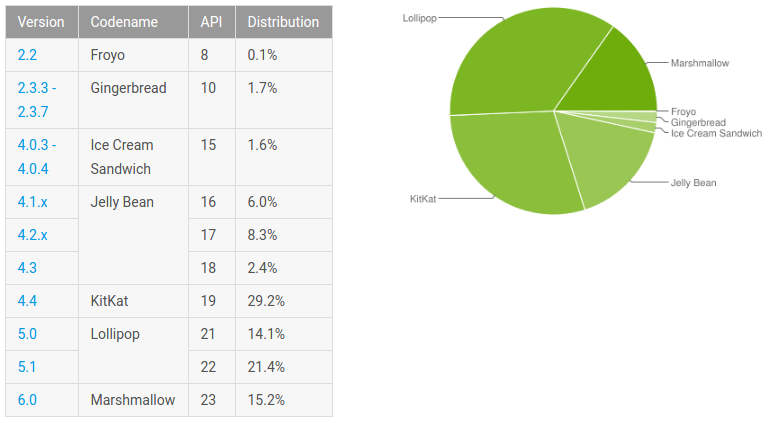
\includegraphics[width=1\textwidth]{imagens/platform_versions.png}
\caption{Distribuição por versão da plataforma \cite{Dashboard}}
\label{fig:platform_versions}
\end{figure}

\subsubsection{Múltiplas Telas}
A plataforma Android oferece suporte para uma variedade de tamanho de tela e faz
a maioria do trabalho para adaptar o layout das aplicações para preencher cada tela
adequadamente. A base para o suporte a múltiplas telas é a habilidade de renderizar
o layout das aplicações redimensionando-os para se adequar ao tamanho da tela e
redimensionando imagens para a densidade da tela. Para melhor adequação às diferentes
telas, desenvolvedores devem também: (i) explicitamente declarar em arquivos de
configuração quais tamanhos de tela suas aplicações suportam; (ii) fornecer diferentes
layouts para diferentes telas através do nome do diretório onde os arquivos são
armazenados (ex: layout-sw600dp – para um layout de 600dp); e (iii) fornecer
imagens de tamanhos diferentes para telas de densidades diferentes. Outra opção
para suportar variedades de telas diferentes é o reuso de fragmentos da interface
do usuário na composição da configuração de layouts diferentes, geralmente
otimizadas para ocupar todo o espaço disponível na tela. A ideia é compor o
layout em tempo de execução. Por exemplo, em um dispositivo pequeno, o adequado
é mostrar apenas um fragmento por vez em uma interface com um único painel.
Por outro lado, considerando dispositivos maiores, pode ser mais apropriado alocar
fragmentos lado-a-lado, exibindo mais informações para o usuário.

A figura \ref{fig:screen_configuration} exibe informações acerca do uso de configuração de tela.
Uma configuração de tela é uma combinação do tamanho da tela e sua densidade -
a quantidade de pixels por área física da tela. Esses valores representando os
dispositivos com Android que acessaram a Google Play Store nos 7 dias anteriores
a 1º de agosto de 2016. Os tamanhos de telas são distribuídos nos valores:
Small, Normal, Large e Xlarge; enquanto a densidade pode assumir: ldpi, mdpi,
tvdpi, hdpi, xdpi e xxdpi.

\begin{figure}[ht]
\centering
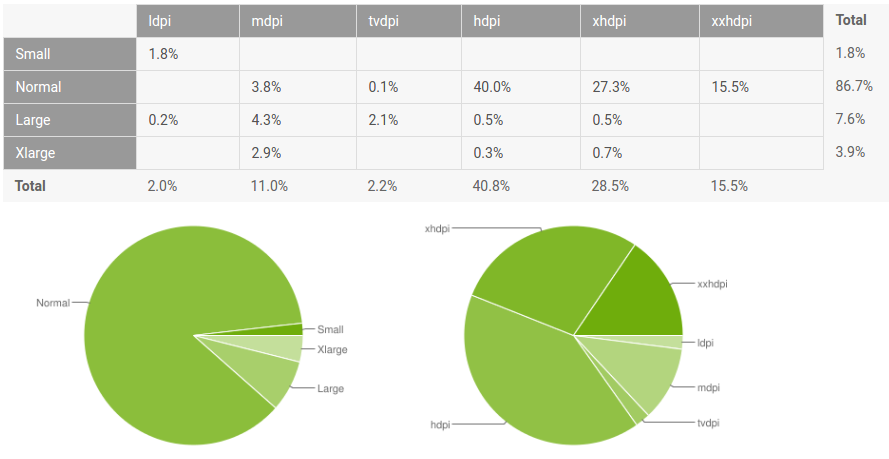
\includegraphics[width=1\textwidth]{imagens/screen_configuration.png}
\caption{Distribuição do uso de configuração de telas \cite{Dashboard}}
\label{fig:screen_configuration}
\end{figure}

\subsubsection{Localização}

A principal forma de localizar aplicativos (adequá-lo para um idioma e cultura de um país)
é fornecendo textos alternativos para diferentes idiomas. Desenvolvedores podem
também disponibilizar imagens, sons, vídeos e outros recursos alternativos.
Para adaptar a localização de aplicativos, a plataforma Android busca por um
diretório com os recursos específicos para a localização. Nesse caso, o nome do
diretório deve ser padronizado, especificando um idioma ou uma combinação de
idioma-região de acordo com seu conteúdo. Em tempo de execução, baseado na
configuração de local do dispositivo, a plataforma Android usa o conjunto de
recursos presente no diretório apropriado. Essa solução é semelhante a já conhecida
e bastante utilizada do GNU gettext\footnote{Disponível em https://www.gnu.org/software/gettext/}
para tratar esse tipo de variabilidade.

\subsubsection{Compatibilidade de Dispositivos}

É bem conhecido que nem todo dispositivo dispõe de todas funcionalidades, assim,
em adição a prover uma interface de usuário flexível que se adapta a configuração
de telas diferentes, aplicações Android também devem ser tolerantes a: (i) alguma
variabilidade de hardware, como a presença ou não de um sensor; (ii) variabilidade
de software, como um widget específico. A plataforma provê mecanismos para detectar
em tempo de execução a presença ou ausência desses elementos.

\section{Padrões de Projeto e Orientação a Objetos}
Padrões de projeto \cite{Gamma1994} e técnicas de orientação a objetos – polimorfismo,
herança, composição, agregação/delegação – são abordagens utilizadas para implementação
de variabilidades de uma forma geral. Padrões de projeto identificam aspectos do sistema
que podem variar e fornecem soluções para gerenciar a variação. Técnicas de OO
são utilizadas para a implementação dos padrões de projeto \cite{Gacek2001}.
Com efeito, há relatos do uso de tal abordagem em linhas de produto de software Android \cite{Pavlic2013}.

\section{Framework para comparação de técnicas de implementação de variabilidades}
Existem diversas técnicas para implementação de variabilidades, de forma que se
faz necessários critérios de comparação e seleção de qual utilizar em uma determinada
situação. \citeonline{Alves2007} propôs um \textit{framework} para comparação de tais técnicas.
O \textit{framework} é uma extenção de outros trabalhos \cite{Gacek2001} \cite{Coplien1999},
cujos critérios de avaliação e valores possíveis estão apresentados na Tabela \ref{tab:framework}.

\begin{table}[h]
  \caption{Framework para comparação de técnicas de implementação de variabilidades}
  \begin{tabular}{ | l | l |}
    \hline
    \textbf{Critério de avaliação} & \textbf{Valores possíveis}  \\ \hline
    Tipo de variabilidade & Positivo, negativo ou ambos  \\ \hline
    Variabilidade na estrutura & Oferece suporte ou não oferece suporte \\ \hline
    Variabilidade no comportamento & Oferece suporte ou não oferece suporte \\ \hline
    Granularidade & Fina ou grossa \\ \hline
    Tempo de ligação & Pré-processamento, compilação, implantação, execução \\ \hline
    Reusabilidade & Alta, média, ou baixa \\ \hline
    Legibilidade & Alta, média, ou baixa \\ \hline
    Desempenho & Alta, média, ou baixa \\ \hline
    Tamanho da aplicação & Alto impacto ou baixo impacto \\ \hline
    \begin{tabular}[c]{@{}l@{}}Suporte para implementação\\ modular de requisitos transversais\end{tabular}  & Oferece suporte ou não oferece suporte \\ \hline
  \end{tabular}
  \label{tab:framework}
\end{table}

\textbf{Tipo de variabilidade} indica a adição ou remoção de comportamento ou
estrutura quando comparada com uma implementação base. \textbf{Variabilidade na estrutura}
indica a possibilidade de estaticamente organizar elementos do programa, como adição
de métodos ou atributos em, enquanto
\textbf{variabilidade no comportamento} diz respeito a diferentes semânticas de execução.
\textbf{Granularidade fina} refere-se a variações em nível de métodos de classe,
incluindo trechos no corpo dos metodos, ao passo que \textbf{granularidade grossa}
é uma variação em nível de classes. \textbf{Tempo de ligação} indica o momento
durante o desenvolvimento em que as decisões acerca da variação tem que ser tomada,
por exemplo, uma variação pode ser tratada durante a compilação ou somente no momento da execução.

Outros parâmetros importantes para avaliação são \textbf{reusabilidade}, \textbf{legibilidade}, 
\textbf{tamanho da aplicação} e \textbf{desempenho}, esses dois últimos dizem
respeito a um produto executável da LPS. 

Também é considerado o \textbf{suporte para implementação modular de requisitos transversais}.
Esse suporte é importante porque muitas variabilidades de LPS podem ser requisitos transversais,
como apontado por diversas pesquisas \cite{Gacek2001} \cite{Batory2004} \cite{Liu2006}
\cite{Lopez2005} \cite{mezini2004}.

